% !TEX TS-program = pdflatex
% !TEX encoding = UTF-8 Unicode

% This is a simple template for a LaTeX document using the "article" class.
% See "book", "report", "letter" for other types of document.

\documentclass[11pt]{article} % use larger type; default would be 10pt

\usepackage[utf8]{inputenc} % set input encoding (not needed with XeLaTeX)
\usepackage{wrapfig}
%%% Examples of Article customizations
% These packages are optional, depending on whether you want the features they provide.
% See the LaTeX Companion or other references for full information.

%%% PAGE DIMENSIONS
\usepackage{geometry} % to change the page dimensions
\geometry{a4paper} % or letterpaper (US) or a5paper or....
% \geometry{margin=2in} % for example, change the margins to 2 inches all round
% \geometry{landscape} % set up the page for landscape
% read geometry.pdf for detailed page layout information

\usepackage{graphicx} % support the \includegraphics command and options
\usepackage{url} % better links representation, o così dicono

% \usepackage[parfill]{parskip} % Activate to begin paragraphs with an empty line rather than an indent

%%% PACKAGES
\usepackage{booktabs} % for much better looking tables
\usepackage{array} % for better arrays (eg matrices) in maths
\usepackage{paralist} % very flexible & customisable lists (eg. enumerate/itemize, etc.)
\usepackage{verbatim} % adds environment for commenting out blocks of text & for better verbatim
\usepackage{subfig} % make it possible to include more than one captioned figure/table in a single float
% These packages are all incorporated in the memoir class to one degree or another...
\usepackage{listings}

\usepackage{graphicx}
\graphicspath{ {./images/} }

%%% HEADERS & FOOTERS
\usepackage{fancyhdr} % This should be set AFTER setting up the page geometry
\pagestyle{fancy} % options: empty , plain , fancy
\renewcommand{\headrulewidth}{0pt} % customise the layout...
\lhead{}\chead{}\rhead{}
\lfoot{}\cfoot{\thepage}\rfoot{}

%%% SECTION TITLE APPEARANCE
\usepackage{sectsty}
\allsectionsfont{\sffamily\mdseries\upshape} % (See the fntguide.pdf for font help)
% (This matches ConTeXt defaults)

\usepackage[usenames,dvipsnames]{xcolor}
\usepackage{hyperref} % To refer a link (website)
\hypersetup{%
  colorlinks=true,% hyperlinks will be coloured
  %linkcolor={BrickRed},% hyperlink text will be green
  linkbordercolor=BrickRed,
  citebordercolor=White,
  urlbordercolor=White,
  runbordercolor=White,
  menubordercolor=White,
  filebordercolor=White,
 % urlcolor={BrickRed},
%filecolor={White},
%citecolor={BrickRed},
allcolors={BrickRed}
%allbordercolors={BrickRed}
}

\makeatletter
\Hy@AtBeginDocument{%
  \def\@pdfborder{0 0 1}% Overrides border definition set with colorlinks=true
  \def\@pdfborderstyle{/S/U/W .5}% Overrides border style set with colorlinks=true
                                % Hyperlink border style will be underline of width 1pt
}
\makeatother

%%% ToC (table of contents) APPEARANCE
\usepackage[nottoc,notlof,notlot]{tocbibind} % Put the bibliography in the ToC
\usepackage[titles,subfigure]{tocloft} % Alter the style of the Table of Contents

\renewcommand{\cftsecfont}{\rmfamily\mdseries\upshape}
\renewcommand{\cftsecpagefont}{\rmfamily\mdseries\upshape} % No bold!

\setlength\parindent{0pt} % Set noindent for the whole document
\newcommand{\ES}{\textcolor{red}}


\usepackage{tikz}
\usetikzlibrary{shapes,trees,fit,decorations.pathreplacing,arrows.meta}


%%% END Article customizations

\begin{document}
%\maketitle

%%% Title page
\begin{titlepage}
	\topskip0pt
	%\vspace*{\fill}
	\centering
	
\includegraphics[width=\textwidth]{logo.png}\\
	\vspace*{1cm}
	\Large \textsc{Corso di Laurea Magistrale in Informatica}
	
	\vspace*{10mm}
	\hrule width \hsize \kern 1mm \hrule width \hsize height 2pt
	\vspace*{5mm}
	\Huge \emph{\textbf{Asset Language}}\\
	\large \emph{\textbf{Compilers and Interpreters Project}}\\
	\large \emph{\textbf{Report on design choices}}
	\vspace*{5mm}
	\hrule width \hsize height 2pt
	\vspace*{1mm}
	\hrule width \hsize \kern 1mm
	
	\vspace*{10mm}
	\begin{minipage}{0.45\textwidth}
		\begin{flushleft} \Large
			\emph{Students:}\\
			\Large \textbf{Alberto \textsc{Paparella}}
			\Large \textbf{Giuseppe \textsc{Caputo}}\\
			\Large \textbf{Gabriele \textsc{Spina}}
		\end{flushleft}
	\end{minipage}	
	\begin{minipage}{0.45\textwidth}
		\begin{flushright} \Large
			\emph{Professor:}\\
			\Large \textbf{Prof. Cosimo \textsc{Laneve}}
		\end{flushright}
	\end{minipage}
	
	\vspace*{15mm}
	\Large \textsc{Academic Year $2021-2022$}
\end{titlepage}

% Table of contents
\addtocontents{toc}{~\hfill\textbf{Page}\par}	% https://texblog.org/2011/09/09/10-ways-to-customize-tocloflot/
\pagestyle{empty}
\clearpage
\tableofcontents
\thispagestyle{empty}
\addtocontents{toc}{\protect\thispagestyle{empty}}	% http://tex.stackexchange.com/questions/2995/removing-page-number-from-toc
\newpage

\section{Introduction}
This report will discuss and illustrate the implementation choices related to the design of a compiler for a specific programming language called \emph{AssetLan} (i.e., Asset Language). 

\medskip

\emph{Asset Language} is a simple imperative language with asset, where parameters could be either {\emph standard} or {\emph asset}, with recursion and without mutual recursion. Regarding the semantics, two types of operations are allowed on a parameter defined as {\emph asset}, and it is legit use them only in a function. To this aim, the functions could be declared  with {\emph asset} in that way:\begin{verbatim}
void f(int a, bool b)[asset u, asset v] { body }
\end{verbatim} 
and called as: 
\begin{verbatim}
f(5,true)[x,y]
\end{verbatim}
At the time of the call, assets 'x' and 'y' are emptied, and their values are assigned respectively to the formal parameters 'u' e 'v', so after the call 'x' and 'y' values are 0.

\medskip

The value of an \emph{asset} can be \textbf{only} moved using the aforementioned 2 operations, more in specific: 
\begin{itemize}
\item \textbf{Move} (\emph{x -o z}) : the result of that operation is that the value of the first parameter is summed to the second one, and then it is cleaned (set to 0). This operation, as the following one, is legit only with 2 asset arguments.
\item \textbf{Transfer} (\emph{transfer x}) : this operation transfer the value of the \emph{asset} 'x' to the caller of the function, and so it became 0.
\end{itemize}

\section{Exercises}
\label{sec:exercices}
The following exercises were used as guidelines/objectives for the design 
blabalbalbal

\begin{enumerate}
\item \textbf{Lexical Errors} : the lexical analyzer must return the list of lexical errors in an output file. 
\item \textbf{Symbol Table} : implement the table of symbols as list of hash-table or hash-table of lists. In order to check errors related to:
\begin{itemize}
\item undeclared functions/variables;
\item multiple declarations of functions/variables in the same environment;
\end{itemize}
\end{enumerate}

\subsection{Lexical Errors}
In order to redirect the errors of the lexer to an output (log) file, we must override the base error handling strategy of ANTLR, because by default it sends the errors to the standard error (i.e., the console). To change the destination and, if desired, the content of the errors messages one must provide an implementation of interface \textsc{ANTLRErrorListener}, in Figure~\ref{fig:err} is illustrated the structure of the classes involved in error handling phase.
\begin{figure}
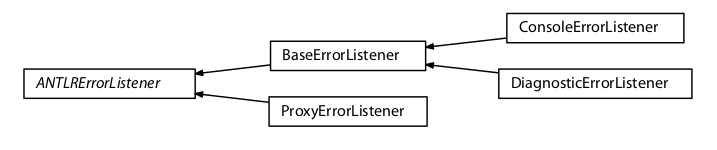
\includegraphics[width=\textwidth]{errorListener.png}
\caption{Internal structure for error handling.}
\label{fig:err}
\end{figure}   
\textsc{ANTLRErrorListener} has a \textsc{syntaxError()} method that applies both lexers and parsers, it receives all sorts of information about the location of the error as well as the error message.     

\medskip

The proposed solution consists in a class called \textsc{TestLexerListner} that extends the \textsc{BaseErrorListner} class in order to override the \textsc{syntaxError()} method and redirect his output to a log file, called \textsc{log.txt}. In addition, for each error, has been added the time at which it occurred, so that it is possible to distinguish errors coming from different compilation executions. 

\medskip

Now a test application can be implemented, it must remove the \textsc{ConsoleErrorListener} (i.e., the default strategy), and add the custom one. After that we can do the parse phase as usual.

A lexical errror is a sequence of characters that does not match the pattern of any token.
\ES{DISCUTERE I 3 ERRORI}
%\lstinputlisting[language=Java]{TestLexerListener.java}


\subsection{Symbol Table}
The choice of the data structure for the symbol table fell on the list of hash-table, because an excessive level of nesting in the code is not expected. This can be said due to the fact that the grammar of the language does not allow the definition of code blocks, so the only way to enter in a new scope/environment is the definition of a function or an if-then-else statement. 

\medskip

The symbol table has been declared as a private field in a specific class called \textsc{Environment}. In order to access/modify it, has been implemented a certain number of methods:
\begin{itemize}
\item \textsc{enterScope()} : increase the nesting level and add a new entry (i.e., an hash-table) to the list. 
\item \textsc{exitScope()} : decrease nesting level and remove the last hash-table in the list.
\item \textsc{getScope()}/\textsc{getCurrentScope()} : get the scope of current nesting level or of a specified one.
\item \textsc{addEntry} : add an entry to the current scope.
\item \textsc{getNestingLevel()} : getter for nesting level field.
\item \textsc{checkDeclaration()} : checks if the symbol has been declared in this scope. 
\end{itemize}

\medskip

To manage the symbol table, it is necessary to visit the AST in order to insert the declarations of variables / functions / assets within the data structure. To this aim, it has been extended the \textsc{AssetLanBaseVisitor} class to override the methods auto-generated meant to visit the AST. For each rule of the grammar, it has been defined a new class representing a node of the tree with his specific components. Moreover, there are the method to manage this objects and most important the method \textsc{checkSemantics()} that checks for errors specified in Section~\ref{sec:exercices}.

\medskip

In the \textsc{AssetLanBaseVisitor} there is a visit method for each rule of the grammar, the work done on each one of this consisted in the construction of the related node with the help of the ANTLR's rule contexts. 


\end{document}
